\chapter{Results}
\section*{Mean Square Error}
In statistics, the mean squared error (MSE) is used to calculate the average of the squares of the errors. It
mean that the difference between the estimator and what is estimated.
The MSE is one of quality evaluation method. In this internship, it help us to know best result when it is the smallest.
 





\

\begin{center}

	$MSE =  \dfrac{1}{n} \displaystyle \sum_{i=1}^{n}(\hat{Y_i} - Y_i)^2$
	

\end{center}
\vspace{3cm}

\section*{Peak signal to noise ratio}
The PSNR is also one of quality evaluation method. In this internship, it help us to know best result when it is the biggest. 

\vspace{1cm}

\begin{center}
	
	$PSNR = 10\log_{10}\left(\dfrac{255^2}{MSE}\right)  $
	
	
\end{center}
\newpage
\section*{Lena Image}
\begin{center}

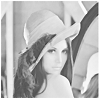
\includegraphics{lena.png}



\vspace{1cm}	
Lena.tif 

\begin{tabular}{|c|c|c|}
	\hline 
	Filter & MSE & PSNR \\ 
	\hline 
	Median & 0.0372 & 62.4258 \\ 
	\hline 
	Average & 0.0184 & 65.4860 \\ 
	\hline 
	Gaussian & 0.0041 & 72.0197 \\ 
	\hline 
	Weiner & 0.0366 & 62.4964 \\ 
	\hline 
	%SURE-LET & 3.22 & 43.05 \\ 
%	\hline 
\end{tabular} 

\

Comparison Table
\end{center}
\vspace{3cm}

\section*{Cameraman Image}
\begin{center}
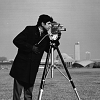
\includegraphics{cameraman.png}

\vspace{1cm}	
	Cameraman.tif
	
	\begin{tabular}{|c|c|c|}
		\hline 
		Filter & MSE & PSNR \\ 
		\hline 
		Median & 0.1060 & 57.8789 \\ 
		\hline 
		Average & 0.0145 & 66.5120 \\ 
		\hline 
		Gaussian & 0.0059 & 70.3933 \\ 
		\hline 
		Weiner & 0.1148 & 57.5314 \\ 
		\hline 
		%SURE-LET & 3.22 & 43.05 \\ 
		%\hline 
	\end{tabular} 
	
	\
	
	Comparison Table
\end{center}
\vspace{3cm}

\section*{Coco Image}
\begin{center}
	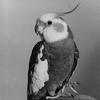
\includegraphics{coco.png}
	
	\vspace{1cm}
	Coco.tif
	
	\begin{tabular}{|c|c|c|}
		\hline 
		Filter & MSE & PSNR \\ 
		\hline 
		Median & 0.0684 & 59.7830 \\ 
		\hline 
		Average & 0.0096 & 68.3246 \\ 
		\hline 
		Gaussian & 0.0016 & 75.9843 \\ 
		\hline 
		Weiner & 0.0762 & 59.3135 \\ 
		\hline 
		%SURE-LET & 2.23 & 44.64 \\ 
		%\hline 
	\end{tabular} 
	
	\
	
	Comparison Table
\end{center}
\vspace{3cm}

\section*{House Image}
\begin{center}
	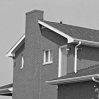
\includegraphics{house.png}
	
	\vspace{1cm}
	House.tif
	
	\begin{tabular}{|c|c|c|}
		\hline 
		Filter & MSE & PSNR \\ 
		\hline 
		Median & 0.0521 & 60.9607 \\ 
		\hline 
		Average & 0.0132 & 66.9250 \\ 
		\hline 
		Gaussian & 0.0027 & 73.7704 \\ 
		\hline 
		Weiner & 0.0580 & 60.4962 \\ 
		\hline 
	%	SURE-LET & 2.77 & 43.70 \\ 
	%	\hline 
	\end{tabular} 
	
	\
	
	Comparison Table
\end{center}
\vspace{3cm}

\section*{Peppers Image}
\begin{center}
\includegraphics{Peppers.png}	
	
	\vspace{1cm}
	Peppers.tif
	
	\begin{tabular}{|c|c|c|}
		\hline 
		Filter & MSE & PSNR \\ 
		\hline 
		Median & 0.0827 & 58.9580 \\ 
		\hline 
		Average & 0.0105 & 67.9129 \\ 
		\hline 
		Gaussian & 0.0040 & 72.1321 \\ 
		\hline 
		Weiner & 0.0908 & 58.5492 \\ 
		\hline 
	%	SURE-LET & 3.17 & 43.13 \\ 
	%	\hline 
	\end{tabular} 
	
	\
	
	Comparison Table
\end{center}
\vspace{1cm}

Normally paper in the chapter 2 as we see, they usually use PSNR or MSE to quality comparison of image after denoise. But in this report, we used 2 methods to obtain best result and showed best noise removal method. With 5 images above, value comparison by MSE and PSNR. We have best of results Gaussian filter with MSE is minimum mean square error and it is maximum PSNR.


%This part must contain the result of the method/algoritm/system developed during the internship. \\

%This part must also include comparisons with the state of the art.\\

%Use tables, figures, graphics to illustrate your results. \\ 

%Comment your results, and explain the context used to obtain these results.




